% \documentclass[a4paper, conference, compsoc]{IEEEtran}
\documentclass[12pt,a4paper,colorinlistoftodos]{article}
% \documentclass[%
%     pdftex,
%     oneside,			% Einseitiger Druck.
%     12pt,				% Schriftgroesse
%     parskip=half,		% Halbe Zeile Abstand zwischen Absätzen.
% %	topmargin = 10pt,	% Abstand Seitenrand (Std:1in) zu Kopfzeile [laut log: unused]
%     headheight = 12pt,	% Höhe der Kopfzeile
% %	headsep = 30pt,	% Abstand zwischen Kopfzeile und Text Body  [laut log: unused]
%     headsepline,		% Linie nach Kopfzeile.
%     footsepline,		% Linie vor Fusszeile.
%     footheight = 16pt,	% Höhe der Fusszeile
%     abstracton,		% Abstract Überschriften
%     DIV=calc,		% Satzspiegel berechnen
%     BCOR=8mm,		% Bindekorrektur links: 8mm
%     headinclude=false,	% Kopfzeile nicht in den Satzspiegel einbeziehen
%     footinclude=false,	% Fußzeile nicht in den Satzspiegel einbeziehen
%     listof=totoc,		% Abbildungs-/ Tabellenverzeichnis im Inhaltsverzeichnis darstellen
%     toc=bibliography,	% Literaturverzeichnis im Inhaltsverzeichnis darstellen
% ]{scrreprt}	% Koma-Script report-Klasse, fuer laengere Bachelorarbeiten alternativ auch: scrbook


% Basic packages
\usepackage[T1]{fontenc}
\usepackage[utf8]{inputenc}
\usepackage[scaled]{beramono}
\usepackage[english,ngerman]{babel,varioref}
\usepackage{xcolor}
\usepackage{amsmath}

% Tables
\usepackage{booktabs}
\usepackage{multirow}
\usepackage{longtable}
% Graphics and Includes
\usepackage[pdftex]{graphicx}
\graphicspath{{assets/img/}}
\DeclareGraphicsExtensions{.pdf,.jpeg,.png,.jpg}
\usepackage{tikz}
\usetikzlibrary{arrows.meta,bending,automata,shapes}
\usepackage[underline=true,rounded corners=false]{pgf-umlsd}

% Reduce distance before caption
\usepackage[skip=5pt]{caption}

% DirectoryTree
\usepackage[edges]{forest}

\definecolor{folderbg}{RGB}{124,166,198}
\definecolor{folderborder}{RGB}{110,144,169}
\newlength\Size
\setlength\Size{4pt}
\tikzset{%
  folder/.pic={%
    \filldraw [draw=folderborder, top color=folderbg!50, bottom color=folderbg] (-1.05*\Size,0.2\Size+5pt) rectangle ++(.75*\Size,-0.2\Size-5pt);
    \filldraw [draw=folderborder, top color=folderbg!50, bottom color=folderbg] (-1.15*\Size,-\Size) rectangle (1.15*\Size,\Size);
  },
  file/.pic={%
    \filldraw [draw=folderborder, top color=folderbg!5, bottom color=folderbg!10] (-\Size,.4*\Size+5pt) coordinate (a) |- (\Size,-1.2*\Size) coordinate (b) -- ++(0,1.6*\Size) coordinate (c) -- ++(-5pt,5pt) coordinate (d) -- cycle (d) |- (c) ;
  },
}
\forestset{%
  declare autowrapped toks={pic me}{},
  pic dir tree/.style={%
    for tree={%
      folder,
      font=\ttfamily,
      grow'=0,
    },
    before typesetting nodes={%
      for tree={%
        edge label+/.option={pic me},
      },
    },
  },
  pic me set/.code n args=2{%
    \forestset{%
      #1/.style={%
        inner xsep=2\Size,
        pic me={pic {#2}},
      }
    }
  },
  pic me set={directory}{folder},
  pic me set={file}{file},
}
% Bibliography
\usepackage[backend=biber, isbn=false, doi=false, style=ieee]{biblatex}
\addbibresource{bibliography.bib}
\AtBeginBibliography{\raggedright}
%\nocite{*}

% Gossar z.a. für acronyme
% \usepackage[acronym]{glossaries}
% \makeglossaries
\usepackage[printonlyused]{acronym} % falls gewünscht kann die Option footnote eingefügt werden, dann wird die Erklärung nicht inline sondern in einer Fußnote dargestellt

% \section*{Abkürzungsverzeichnis}
\begin{acronym}[AAAAAAA]
    \acro{wysiwyg}[WYSIWYG]{What you see is what you get}
\end{acronym}

% Colors
\definecolor{ListingBackground}{HTML}{E6E6E6}
\definecolor{LinkColor}{HTML}{000000}


% Font
\usepackage[onehalfspacing]{setspace}
\usepackage{lmodern}
\usepackage[official]{eurosym}
\usepackage{enumitem}
\usepackage[locale=DE]{siunitx} % SI Units für Währungen
\DeclareSIUnit{\EUR}{\text{\euro}} % Beispielverwendung: \SI{10.10}{\EUR}

\usepackage[autostyle=true,german=quotes]{csquotes}
\usepackage{url}
\newcommand{\code}[1]{\texttt{#1}}

% Keine Einrückungen am Zeilenanfang
\setlength\parindent{0pt}

% Additional Setup
\usepackage[unicode=true,hypertexnames=false,colorlinks=true,linkcolor=LinkColor,citecolor=LinkColor,urlcolor=LinkColor,pdftex]{hyperref}

% Trennung von URLs im Literaturverzeichnis (große Werte [> 10000] verhindern die Trennung)
\defcounter{biburlnumpenalty}{10} % Strafe für Trennung in URL nach Zahl
\defcounter{biburlucpenalty}{500}  % Strafe für Trennung in URL nach Großbuchstaben
\defcounter{biburllcpenalty}{500}  % Strafe für Trennung in URL nach Kleinbuchstaben
\interfootnotelinepenalty=10000 % prevent all footnotes from breaking over a page.

% Configs
\setcounter{tocdepth}{1} % Limit table of contents to subsection
\sisetup{detect-weight=true, detect-family=true} % SI Units shall detect font weight and family
\setlist[description]{style=nextline} % Break definitions of terms to a new line (used by \begin{description} \item[foo] bar \end{description})
\renewcommand*{\bibfont}{\small}

%Hurenkinder und Schusterjungen vermeiden
\clubpenalty = 10000
\widowpenalty = 10000
\displaywidowpenalty = 10000

% Quellcode
\usepackage{listings}
\usepackage{float}
\usepackage{textcomp}
\lstset{
    inputpath=assets/listings,
    language=Java,			% Standardsprache des Quellcodes
    numbers=left,			% Zeilennummern links
    stepnumber=1,			% Jede Zeile nummerieren.
    numbersep=5pt,			% 5pt Abstand zum Quellcode
    numberstyle=\tiny,		% Zeichengrösse 'tiny' für die Nummern.
    breaklines=true,		% Zeilen umbrechen wenn notwendig.
    breakautoindent=true,	% Nach dem Zeilenumbruch Zeile einrücken.
    postbreak=\space,		% Bei Leerzeichen umbrechen.
    tabsize=2,				% Tabulatorgrösse 2
    basicstyle=\ttfamily\footnotesize, % Nichtproportionale Schrift, klein für den Quellcode
    showspaces=false,		% Leerzeichen nicht anzeigen.
    showstringspaces=false,	% Leerzeichen auch in Strings ('') nicht anzeigen.
    extendedchars=true,		% Alle Zeichen vom Latin1 Zeichensatz anzeigen.
    captionpos=b,			% sets the caption-position to bottom
    backgroundcolor=\color{ListingBackground}, % Hintergrundfarbe des Quellcodes setzen.
    xleftmargin=0pt,		% Rand links
    xrightmargin=0pt,		% Rand rechts
    frame=single,			% Rahmen an
    frameround=ffff,
    rulecolor=\color{darkgray},	% Rahmenfarbe
    fillcolor=\color{ListingBackground},
    keywordstyle=\color[rgb]{0.133,0.133,0.6},
    commentstyle=\color[rgb]{0.133,0.545,0.133},
    stringstyle=\color[rgb]{0.627,0.126,0.941},
    float,
    upquote=true
}


\colorlet{punct}{red!60!black}
\definecolor{delim}{RGB}{20,105,176}
\colorlet{numb}{magenta!60!black}

\lstdefinelanguage{TypeScript}{
    keywords={typeof, new, true, false, catch, function, return, null, catch,
    switch, var, if, in, while, do, else, case, break, number, string, Date},
    keywordstyle=\color{delim}\bfseries,
    ndkeywords={class, export, boolean, throw, implements, import, this, type, defaults, extends},
    ndkeywordstyle=\color{magenta}\bfseries,
    identifierstyle=\color{black},
    sensitive=true,
    morecomment=[s]{<}{>}, % Actually not a Comment but a Tag
    commentstyle=\color{red}\ttfamily,
    stringstyle=\color{red}\ttfamily,
    morestring=[b]',
    morestring=[b]"
}


\lstdefinelanguage{json}{
    string=[s]{"}{"},
    stringstyle=\color{numb},
    literate=
     *{0}{{{\color{numb}0}}}{1}
      {1}{{{\color{numb}1}}}{1}
      {2}{{{\color{numb}2}}}{1}
      {3}{{{\color{numb}3}}}{1}
      {4}{{{\color{numb}4}}}{1}
      {5}{{{\color{numb}5}}}{1}
      {6}{{{\color{numb}6}}}{1}
      {7}{{{\color{numb}7}}}{1}
      {8}{{{\color{numb}8}}}{1}
      {9}{{{\color{numb}9}}}{1}
      {:}{{{\color{punct}{:}}}}{1}
      {,}{{{\color{punct}{,}}}}{1}
      {\{}{{{\color{delim}{\{}}}}{1}
      {\}}{{{\color{delim}{\}}}}}{1}
      {[}{{{\color{delim}{[}}}}{1}
      {]}{{{\color{delim}{]}}}}{1}
}

\lstdefinelanguage{yaml}{
  identifierstyle=\color{delim},
  sensitive=false,
  comment=[l]{\#},
  commentstyle=\color{purple}\ttfamily,
  stringstyle=\color{numb},
  morestring=[b]',
  morestring=[b]"
}

\lstdefinelanguage{firestoreRule}{
  identifierstyle=\color{delim},
  keywords={},
  otherkeywords={% Operators
    =, ==, /
  },
   % list of keywords
   keywords= [2]{
    service,
    match,
    allow,
    for
  },
  keywordstyle=\color{purple},
  keywordstyle=[2]\color{numb},
  sensitive=false
}

\lstloadlanguages{Python,Java,bash}



% Algorithmen (Pseudocode)
\usepackage[german,onelanguage,linesnumbered,ruled]{algorithm2e}
% Styling Kommentar
\newcommand\mycommfont[1]{\color{gray}\ttfamily{#1}}
\SetCommentSty{mycommfont}

% Runde Klammern um Bedingungen
\SetKwIF{If}{ElseIf}{Else}{wenn~(}{)~dann}{sonst wenn~(}{sonst}{}
\SetKwFor{ForEach}{für jedes~(}{)~tue}{Ende}

%Eingabe und Ausgabe Texte
\SetKwInOut{Input}{Eingabe}
\SetKwInOut{Output}{Ausgabe}
% Useful tools
\usepackage{blindtext}
\usepackage{lipsum}
\usepackage[section]{placeins} % Prevent figures and tables to float to new section

\usepackage[]{todonotes}
\newcommand{\todoask}[2][]
{\todo[color=green, #1]{#2}}

\usepackage[normalem]{ulem}

%Angaben zur Arbeit
\def\myTitel{Time Manager (Arbeitstitel)}
\def\myArbeit{Programmentwurf}
\def\myFach{Mobile Computing}
\def\myDatum{\today}
\def\myBetreuer{ÄNDERE MICH!!!}
\def\myGutachter{Strenger Gutachter}
\def\myBearbeitungszeit{Lange}
\def\myAbgabeort{Heilbronn}

%Angaben zur Person
\def\myAutorA{Daniel Knecht}
\def\myAutorB{Lea Poletin}

\def\myDegree{Master Informatik}
\def\myInstitution{DHBW CAS, Bildungscampus 13, 74076 Heilbronn}
\def\myMatrikelnrA{6311764}
\def\myMatrikelnrB{8514262}
\def\myKurs{TMINF17}
\def\myFirma{SAP SE}
\def\myFirmenort{Walldorf}
%\section*{Abkürzungsverzeichnis}
\begin{acronym}[AAAAAAA]
    \acro{wysiwyg}[WYSIWYG]{What you see is what you get}
\end{acronym}

\begin{document}



\title{\myTitel}
\author{\myAutorA~(\myMatrikelnrA), \myAutorB~(\myMatrikelnrB)\\
    \small{\myFach}\\
    \small{\myDegree}\\
    \small{\myInstitution}
}
\date{\myDatum}

\begin{titlepage}
	\begin{longtable}{p{8.2cm} p{5.4cm}}
		% Firmenlogo
		&
		
\includegraphics[width=5.4cm]{casLogo}
	\end{longtable}
	\addtocounter{table}{-1}
    {\let\newpage\relax\maketitle}
    \thispagestyle{empty}
    % \vfill
    \begin{abstract}
Diese Seminararbeit beschreibt die Konzeptentwicklung, Designentscheidungen und Entwicklung
einer Zeitmanagement-App mit dem Arbeitstitel \textit{Time Manager}. 
Für die Entwicklung wurden aktuelle Technologien wie React-Native, Redux, Redux-Saga und 
Firebase verwendet. Die App hat das Ziel das Zeitmanagement während eines Dualen Studiums zu 
vereinfachen. Für den Benutzer soll der Aufwand für das Erfassen neuer Zeiten möglichst gering sein, 
und dementsprechend angepasste Funktionalitäten bieten.
\end{abstract}
\end{titlepage}
% \begin{titlepage}
	\begin{longtable}{p{8.2cm} p{5.4cm}}
		% Firmenlogo
		&
		
\includegraphics[width=5.4cm]{casLogo}
	\end{longtable}
	\addtocounter{table}{-1}
	\enlargethispage{20mm}
	\begin{center}
		\vspace*{12mm}	{\LARGE\textbf \myTitel }\\
		\vspace*{12mm}	{\large\textbf \myArbeit}\\
		% \vspace*{12mm}	\langdeckblattabschlusshinleitung\\
		\vspace*{3mm}		{\textbf \myDegree}\\
		\vspace*{12mm}	des Studiengangs \myKurs\\
    \vspace*{3mm}		am DHBW CAS\\
		\vspace*{12mm}	von\\
		\vspace*{3mm}		{\large\textbf \myAutor}\\
		\vspace*{12mm}	\myDatum\\
	\end{center}
	\vfill
	\begin{spacing}{1.2}
	\begin{tabbing}
		mmmmmmmmmmmmmmmmmmmmmmmmmm             \= \kill
		\textbf{Bearbeitungszeit}       \>  \myBearbeitungszeit\\
		\textbf{Matrikelnummer, Kurs}  \>  \myMatrikelnr, \myKurs\\
		\textbf{Firma}                  \>  \myFirma, \myFirmenort\\
		\textbf{Betreuer}               \>  \myBetreuer\\
		\textbf{Gutachter}              \>  \myGutachter
	\end{tabbing}
	\end{spacing}
\end{titlepage}

\pagenumbering{Roman}

% Sperrvermerk
% \thispagestyle{empty}
% Sperrvermerk direkt hinter Titelseite
\section*{Sperrvermerk}

\vspace*{2em}

Die vorliegende {\myArbeit} mit dem Titel {\itshape{} \myTitel{}\/}
enthält unternehmensinterne bzw. vertrauliche Informationen der {\myFirma},
ist deshalb mit einem Sperrvermerk versehen
und wird ausschließlich zu Prüfungszwecken am Studiengang
{\myDegree} der Dualen Hochschule Baden-Württemberg vorgelegt.
Sie ist ausschließlich zur Einsicht durch den zugeteilten Gutachter,
die Leitung des Studiengangs und ggf. den Prüfungsausschuss des Studiengangs
bestimmt.  Es ist untersagt,
\begin{itemize}
\item den Inhalt dieser Arbeit (einschließlich Daten, Abbildungen, Tabellen, Zeichnungen usw.) als Ganzes oder auszugsweise weiterzugeben,
\item Kopien oder Abschriften dieser Arbeit (einschließlich Daten, Abbildungen, Tabellen, Zeichnungen usw.) als Ganzes oder in Auszügen anzufertigen,
\item diese Arbeit zu veröffentlichen bzw. digital, elektronisch oder virtuell zur Verfügung zu stellen.
\end{itemize}
Jede anderweitige Einsichtnahme und Veröffentlichung – auch von Teilen der Arbeit – bedarf der vorherigen Zustimmung durch den Verfasser und {\myFirma}.

\vspace{3em}

\myAbgabeort, \myDatum
\vspace{4em}

\rule{6cm}{0.4pt}\\
\myAutor

% \newpage

% Erklärung
\thispagestyle{empty}

\section*{Selbstständigkeitserklärung}
\vspace*{2em}


Wir versichern hiermit,
dass der {\myArbeit} mit dem Thema: {\itshape \myTitel } selbstständig verfasst und keine anderen
als die angegebenen Quellen und Hilfsmittel verwendet wurden.
Wir versichern zudem, dass die eingereichte elektronische Fassung mit der gedruckten Fassung übereinstimmt.


\vspace{3em}
\noindent
\myAbgabeort, \myDatum
\\
\\
\noindent
\begin{tabular}{l l}
\rule{6cm}{0.4pt} &  \rule{6cm}{0.4pt}\\
\myAutorA         &  \myAutorB

\end{tabular}

\newpage


% \begin{abstract}
Diese Seminararbeit beschreibt die Konzeptentwicklung, Designentscheidungen und Entwicklung
einer Zeitmanagement-App mit dem Arbeitstitel \textit{Time Manager}. 
Für die Entwicklung wurden aktuelle Technologien wie React-Native, Redux, Redux-Saga und 
Firebase verwendet. Die App hat das Ziel das Zeitmanagement während eines Dualen Studiums zu 
vereinfachen. Für den Benutzer soll der Aufwand für das Erfassen neuer Zeiten möglichst gering sein, 
und dementsprechend angepasste Funktionalitäten bieten.
\end{abstract}
% \newpage

\pagestyle{plain}		% nur Seitenzahlen im Fuß

% Inhaltsverzeichnis
\begin{spacing}{1.1}
    \begingroup
        \pagestyle{empty}
        %für die Anzeige von Unterkapiteln im Inhaltsverzeichnis
        \setcounter{tocdepth}{2}

        \tableofcontents
        \clearpage
    \endgroup
\end{spacing}
\newpage

% Abkürzungsverzeichnis
% \cleardoublepage
% \section*{Abkürzungsverzeichnis}
\begin{acronym}[AAAAAAA]
    \acro{wysiwyg}[WYSIWYG]{What you see is what you get}
\end{acronym}


% Abbildungsverzeichnis
\cleardoublepage
\listoffigures

%Tabellenverzeichnis
% \cleardoublepage
\listoftables

% Quellcodeverzeichnis
% \cleardoublepage
\lstlistoflistings
\cleardoublepage

% \listoftodos
% \cleardoublepage


\pagenumbering{arabic}

\section{Einleitung}\label{sec:einleitung}

\todo[inline]{Setup}
\todo[inline]{- Warum react-native}
\todo[inline]{- warum ohne expo}
\todo[inline]{- warum Typescript}
\todo[inline]{- warum nicht react-native-firebase}
\todo[inline]{- Warum erst dummy-Projekt --> Einfacher Aufzubauen}


\todo[inline]{Firebase Rules}

\newpage
\section{Entwurf}\label{sec:entwurf}

\subsection{Entscheidungen}
\paragraph{UI-Bibliothek}
Im Unternehmen der beiden Autoren findet zeitgleich zu diesem Programmentwurf durch Kollegen ein Umbau der Web-Applikation hin zu React und Redux statt.
Um Synnergien zu nutzen und einen Transfer in die Praxis zu ermöglichen soll daher der Prototyp dieses Programmentwurfs auf ähnlichen Technologien basieren.
Da das Ziel dieses Programmentwurfs eine Mobile Applikation ist, ergeben sich aus dieser Anforderung folgende Möglichkeiten:
\begin{itemize}
    \item (Progressive) Web App mittles React (Web)
    \item Hybride, native App mit React (Web) und PhoneGap
    \item Hybride, native App mit React Native
\end{itemize}

Aus diesen drei Alternativen ist React Native am nächsten an einer nativen Anwendung.
Im Gegensatz zu PhoneGap wird kein Webview in einer nativen Anwendung genutzt um eine Webapp darzustellen,
sondern es werden tatsächliche native UI-Elemente verwendet.
Dadurch fühlt sich die Anwendung nativer an.
Somit fällt hier die Entscheidung auf React Native.

\paragraph{Firebase-Bibliothek}
Da auch die Nutzung von Googles \textit{Firebase}-Plattform bereits als Anforderung gestellt ist,
gilt es auch hier eine Entscheidung zu treffen.

Google bietet zu Nutzung von Firebase verschiedene Bibliotheken an.
Dazu zählen eine Bibliothek für Web- bzw. JavaScript-Anwendungen und eine für Android-Anwendungen.
React Native ist als hybride App jedoch ein Teil von beidem.

Einerseits lässt sich die Web-Bibliothek relativ leicht einbinden.
Andereseits könnten sich Funktionalitäten wie Benachrichtigunen schwieriger gestalten.

Die Android-Bibliothek ist deutlich näher am Gerät, wodurch Gerätefunktionalitäten besser genutzt werden können.
Allerdings besteht hier der Aufwand die Funktionen nativ zu implementieren und in React-Natives-JavaScript zu nutzen.

Das Beste aus diesen beiden Welten verbindet die Bibliothek \textit{React Native Firebase} \cite{invertas78:online}.
Sie stellt eine Zwischenschicht zur Verfügung um auf einfache Weise mit JavaScript-Code auf die native Firebase-Bibliothek zuzugreifen.
Die Bibliothek ist modular aufgebaut, sodass nur die benötigten Funktionalitäten zur Applikation hinzugefügt werden.
Das initiale Einrichten, sowie das hinzufügen bestimmter Module gestaltet sich etwas aufwändiger als die Nutzung der Web-Bibliothek.
Dieses Problem wird jedoch detaillierte Anleitungen kompensiert.

\paragraph{Firebase-Datenbank}
Firebase stellt zwei mögliche Datenbanken zur Verfügung \cite{ChooseaD77:online}.
Die \textit{Realtime Database} ist technisch gesehen ein großes (mehr oder weniger strukturiertes) JSON-Objekt.
Vor allem die Skalierung kann hierbei Problematisch werden.

Im Vergleich dazu werden die Daten im \textit{Cloud Firestore} geordneter dargestellt.
Eine Datenbank besteh aus Sammlungen, welche JSON-ähnliche Dokumente enthalten.
Dokumenten können wiederum Sammlungen enthalten.
Nachteilig am \textit{Cloud Firestore} ist, dass sich dieser noch im Beta-Stadium befindet.
Daher ist es möglich, dass diese Datenbank nicht völlig stabil ist.

Das Ergebnis dieses Programmentwurfs soll keine produktive Applikation, sondern ein Prototyp sein.
Außerdem ist es ein Teilziel neue Technologien anzuwenden.
Aus diesen Gründen wird in dieser Andwendung der \textit{Cloud Firestore} genutzt.

\subsection{Oberflächengestaltung}
Die Gestaltung der Oberflächen orientiert sich an den \textit{Material Design}-Richtlinien von Google.
Auf \cite{DesignMa49:online} werden Richtlinien und Konzepte vorgegeben,
welche Entscheidungen bei der Oberflächengestaltung übernehmen.
Die zudem vorhandene Übersicht an Komponenten lässt sich nutzen um passende Komponenten für einen Anwendungsfall zu finden.

Um erste Ideen für die Oberflächengestaltung zu sammeln,
werden mit Hilfe von dem Tool \textit{Fluid UI} \cite{FluidUIc8:online} sogenannte UI-Mockups erstellt.
Diese Mockups dienen als beispielhafte Vorlage für die spätere Entwicklung.


\begin{figure}[h]
    \centering
    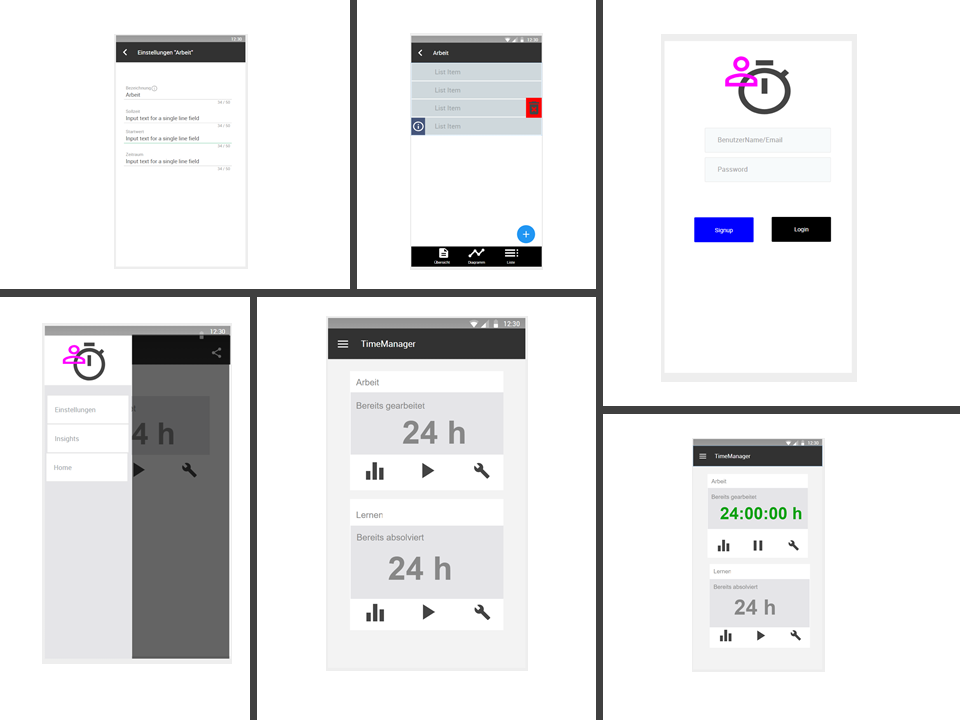
\includegraphics[width=\textwidth]{uiMocks/Mock}
    \caption{UI-Mockups der Anwendung}
\end{figure}




\newpage
\section{Werkzeuge und Technologien (Lea)}
\paragraph{React-Native}

\todo[inline]{Unterschied React, React web React Native}
\todo[inline]{Diagramm Gesamtablauf}
\todo[inline]{- React}
\todo[inline]{- Redux}
\todo[inline]{- Redux-Saga und Firebase}


\paragraph{Typescript}
\todo[inline]{Typescript}
\subsection{Verwendete Bibliotheken}
Im folgenden Abschnitt, werden die in der Applikation verwendetetn Bibliotheken kurz vorgstellt.


\paragraph{react}
\todo[inline]{react}
Komponenten
\paragraph{react-native}
eigentlicher Renderer

\paragraph{react-native-firebase}
\todo[inline]{react-native-firebase}
Firebaseanbindung

\paragraph{react-native-material-dialog}
\todo[inline]{react-native-material-dialog}
Dialog im Material Style

\paragraph{react-navigation}
\todo[inline]{react-navigation}
Navigation im UI
%https://reactnavigation.org/
\paragraph{redux}
\todo[inline]{redux}
state Management

\paragraph{react-redux}

\todo[inline]{react-redux}
Verknüpfung von React und Redux

\paragraph{redux-form}
\todo[inline]{redux-form}
einfache Formulare
Die Bibliothek \textit{redux-form} unterstützt beim Verwalten der Redux-States in Formularen.

\paragraph{redux-saga}
\todo[inline]{redux-saga}
Asynchrone Aktionen

\paragraph{moment}
\textit{Moment.js} ist eine JavaScript-Bibliothek, die das Arbeiten mit Daten vereinfacht. Die Bibliothek ermöglicht es,
ein Datum zu formatieren, validieren und zu manipulieren. Dies ist besonders hilfreich bei der Auswertung und Darstellung der
Zeiterfassung. Das Datum muss hierzu in ein \textit{Moment} umgewandelt werden. \autoref{lst:moment-example} zeigt in einem kleinen Beispiel,
wie die Bibliothek in der Applikation verwendet wurde.
% \lstinputlisting[
%     caption=Beispiel für Moment.js,
%     label=lst:moment-example,
%     language=Typescript,
%     float=ht
% ]{moment.ts}

\paragraph{moment-duration-format}
Dies ist ein Plugin zusätzlich zu \textit{moment.js}. Dieses Plugin in notwendig, da die Dauer ein
grunsätzlich anderes Format hat als ein Datum. Es ermöglicht beispielsweise die Umwandlung einer Anzahl Stunden in Minuten.
In der Applikation wird dieses Format zur Darstellung der Zeiterfassungsergebnisse verwendet.



\paragraph{native-base}
\textit{NativeBase} ist ein Framework, das eine Schicht über React-Native darstellt. Das Framework bietet,
Komponenten für React-Native, die plattformspezifische Designs umsetzen. Diese Komponenten werden für die meisten UI-Komponenten der App
verwendet. %https://nativebase.io/
\newpage
\section{Verzeichnisstruktur}
In \autoref{fig-verzeichnis} sind die ersten zwei Ebenen der Verzeichnisstruktur dargestellt.
Auf die Auflistung automatisch erstellter und nicht veränderter Dateien wird verzichtet.
Der Zweck der Einzelnen Ordner und Dateien wird im Folgenden beschrieben.

\begin{figure}[H]
    \centering
    \begin{forest}
        pic dir tree,
        where level=0{}{% folder icons by default; override using file for file icons
          directory,
        },
      [/
        [App.tsx,file]
        [global.d.ts,file]
        [index.js,file]
        [android]
        [ios]
        [src]
      ]
   \end{forest}
   \begin{forest}
    pic dir tree,
    where level=0{}{% folder icons by default; override using file for file icons
      directory,
    },
    [/src
        [store.ts,file]
        [actions]
        [api]
        [assets]
        [components]
        [container]
        [forms]
        [reducers]
        [sagas]
        [screens]
        [utils]
    ]
\end{forest}
    \caption{Verzeichnisstruktur}
    \label{fig-verzeichnis}
\end{figure}

\paragraph{Oberste Ebene}
\begin{description}
    \item[App.tsx]
    App.tsx ist die Zentrale Datei der Applikation. In ihr wird:
    \begin{itemize}
        \item die Navigation initialisiert,
        \item die Behandlung von Nachrichten eingerichtet,
        \item die Anmeldung des Nutzers sichergestellt,
        \item der Redux-Store mit der App verknüpft.
    \end{itemize}
    \item[global.d.ts]
    Diese Datei wird genutzt um TypeScript-Typen der gesamten Anwendung zur Verfügung zu stellen.
    Hierdurch wird die Arbeit mit komplexeren Datentypen erheblich erleichtert.
    \item[index.js]
    In der Datei wird die Anwendung \enquote{registiert}. Hierdurch werden die React-Native-Componenten mit der nativen Applikation verknüpft.
    Diese automatisch generierte Funktion wird ergänzt durch einen sogenannten \emph{Polyfill}, der genutzt wird,
    um fehlende JavaScript-Funktionalitäten zu ermöglichen. \cite{undefine14:online}
    \item[android]
    Dieser Ordner enthält den Quellcode für die native Android App.
    Wird nativer Code - beispielsweise von React-Native-Firebase - genutzt,
    so muss er hier hinzugefügt werden.
    \item[ios]
    Dieser Ordner ist das Pendant zu vorigem Ordner.
    Da sich dieser Programmentwurf auf Android-Geräte beschränkt,
    bleibt er von manuellen Eingriffen unberührt.
    \item[src]
    In diesem Ordner befindet sich der größte Teil des relevanten Quellcodes.
    Dessen Inhalt wird im folgenden näher betrachtet.
\end{description}

\paragraph{src-Ordner}
Die Aufteilung des \emph{src}-Ordners orientiert sich an dem verbreiteten \emph{Rails-style} \cite{CodeStru4:online}.
Dies bedeutet, dass für jede \enquote{Art} von Bausteinen der Applikation ein eigener Ordner angelegt wird.
Somit ergibt sich folgende Struktur:

\begin{description}
    \item[store.ts]
    In der einzigen Datei direkt im src-Ordner werden die gesamten Reducer zum Redux-Store zusammengefasst und mit
    Redux-Saga verknüpft.
    \item[actions]

    \item[api]
    \item[assets]
    \item[components]
    \item[container]
    \item[forms]
    \item[reducers]
    \item[sagas]
    \item[screens]
    \item[utils]
\end{description}


% \item Codestruktur UI
% \begin{itemize}
%     \item screens
%     \item components
%     \item forms
%     \item container
% \end{itemize}
% \item Codestruktur Redux
% \begin{itemize}
%     \item reducer
%     \item store
%     \item action
% \end{itemize}
% \item Codestruktur Redux-Saga und Firebase
% \begin{itemize}
%     \item sagas
%     \item api
% \end{itemize}

\newpage
\section{Besonderheiten}
\subsection{Firebase}
In dieser Applikation wird Firebase für die Authentifizierung,
die Datenspeicherung, sowie Benachrichtigungen genutzt.
Die ersten beiden Aspekte werden im Folgenden vorgestellt.
Die Benachrichtigungen werden in \autoref{sec:besonderheiten-benachrichtigung} genauer betrachtet.

\paragraph{Authentifizierung}
Die Authentifizierung erfolgt über die von Firebase (bzw. React Native Firebase) zur Verfügung gestellten Schnittstellen.
Jeder Nutzer erhält bei Anmeldung eine UID, über welche er eindeutig identifiziert werden kann.

Firebase unterstützt zur Anmeldung \emph{Anonym, E-Mail/Passwort, Telefon, Google, Play Spiele, Facebook, Twitter} und \emph{GitHub}.
In dieser Anwendung werden die anonyme Anmeldung und die Anmeldung mit E-Mail/Passwort ermöglicht.

\paragraph{Datenspeicherung}
Wie bereits beschrieben, werden die Daten im \textit{Cloud Firestore} gespeichert.
Auf oberster Ebene werden Sammlungen angelegt.
Eine solche Sammlung enthält beliebig viele Dokumente.
Ein Dokument wiederum kann Daten in einem JSON-ähnlichen Format und weitere Sammlungen enthalten.
So lassen sich die gesamte Daten aus wechselnden Sammlungen und Dokumenten strukturieren.

Die Struktur für diesen Programmentwurf ist in \autoref{app-datenbank} dargestellt und wird im Folgenden beschrieben:

Auf oberster Ebene werden unter der Sammlung \texttt{users} alle Benutzer eingeordnet.
Für jeden der Benutzer wird ein Dokument mit dessen UID angelegt.
Dieses Dokument besitzt ein Feld für den Namen des Nutzers,
sowie die Sammlungen \texttt{categories} und \texttt{holidays}.

\texttt{categories} enthält für jede Kategorie ein Dokument mit automatisch generierter ID.
In diesem Dokument befinden sich neben dem Namen alle für die Zeiterfassung relevanten Daten.
Auf diese wird im Verlauf dieser Arbeit genauer eingegangen.
Außerdem enthält eine Kategorie-Dokument die Sammlung \texttt{times}.
Diese wiederum enthält für jede getätigte Zeiterfassung ein Dokument mit Start- und Stoppzeit sowie den gesamten Minuten.

Die Sammlung \texttt{holidays} enthält alle vom Nutzer gepflegten freie Tage mit den notwendigen Informationen.

Um sicherzustellen, dass nur angemeldete Nutzer Zugriff auf ihre Daten haben,
können sogenannte \textit{Regeln} angelegt werden.
Die Regel für diesen Programmentwurf ist in \autoref{lst:firestore-rule} dargestellt.
Über die ersten beiden Zeilen wird die Datenbank adressiert.
Durch die Zeilen 3 und 4 wird geprüft, ob die Nutzer-UID mit dem Titel des Dokuments übereinstimmt.
ist dies der Fall, so werden Lese- und Schreibrechte gestattet.
In Zeile 5 wird durch \lstinline[language=firestoreRule]{**} angegeben,
dass die darauffolgende Regel für alle darunterliegenden Dokumente gilt.
In diesem Fall wird die Regel aus Zeile 4 wiederholt.

\lstinputlisting[
    caption=Regeln für Firestore,
    label=lst:firestore-rule,
    language=firestoreRule,
    float=ht
]{firestoreRule.txt}


Insgesamt besagt die Regel,
dass ein angemeldeter Benutzer auf das zu seinem Benutzer zugehörige Dokument,
sowie alle darunterliegenden Dokumente volle Schreib- und Leseberechtigungen erhält.
Für eine produktive Anwendung könnten diese Regeln noch verschärft werden.
Beispielsweise sind strengere Regeln zur Einhaltung der Datenbankstruktur oder Validierungen der eingegebenen Daten denkbar.
Für die Entwicklung eines Prototyps sind solch strenge Regeln allerdings eher hinderlich.


\subsection{Login}
Die Authentifizierung lässt sich dank Firebase unkompliziert umsetzen.
Auch ein Formular, welches einem Nutzer gestattet sich anzumelden oder zu registrieren ist einfach zu realisieren.

Es bleiben somit noch zwei Aufgaben, welche es zu lösen gilt:
Zum einen sollte ein bereits angemeldeter Benutzer sich an seinem Gerät nicht immer wieder neu anmelden müssen.
Zum anderen sollte der Anwender erst nach Anmeldung Zugriff auf die inneren Funktionen erhalten.

Ersteres ist standardmäßig in React Native Firebase vorgesehen.
Ein Nutzer bleibt auch nach Beenden der App angemeldet.
Beim erneuten Start muss dann überprüft werden, ob bereits ein Nutzer angemeldet ist.
Dies geschieht über die Funktion \texttt{checkLoggedIn} (\autoref{lst:checkLoggedIn}),
welche beim Start der Anwendung aufgerufen wird.
Ist ein Nutzer angemeldet, so wird die Redux-Action \emph{userSignInSuccess},
ansonsten \emph{userSignOutSuccess} gefeuert.
Die Applikation kann dann entsprechend reagieren.

\lstinputlisting[
    caption=checkLoggedIn,
    label=lst:checkLoggedIn,
    language=TypeScript,
    float=ht
]{checkLoggedIn.ts}

Die Komponente \texttt{LoginDeciderComponent} (siehe \autoref{app-LoginDecider}) sorgt dafür,
dass nur angemeldete Nutzer auf die eigentliche Applikation zugreifen können.
Diese Komponente erhält den aktuellen Login-Status aus dem Redux-State und zeigt eine bestimmte Unterkomponente an.
Die Zuordnung zwischen Satus und Unterkomponente ist in \autoref{table:login-states} aufgelistet.
Ein \text{Splash Screen} ist ein einfacher Bildschirm, welcher lediglich das Logo der Anwendung enthält.

\begin{table}[h!]
    \centering
     \begin{tabular}{| l | c | c |}
        \hline
        Status      & Bedeutung                      & Unterkomponente \\
        \hline\hline
        checking    & Prüfung ob Nutzer angemeldet   & Splash Screen\\
        \hline
        logged in   & Nutzer ist angemeldet          & \multirow{2}{*}{Eigentliche Applikation}\\
        \cline{1-2}
        logging out & Nutzer wird abgemeldet         & \\
        \hline
        logged out  & Nutzer ist abgemeldet          & \multirow{2}{*}{Login Screen} \\
        \cline{1-2}
        logging in  & Nutzer wird angemeldet         & \\
        \hline
     \end{tabular}
     \caption{Login Status}
     \label{table:login-states}
\end{table}

Insgesamt wird durch Kombination der beiden Lösungen sichergestellt,
dass ein bereits angemeldeter Nutzer sich nicht nochmals anmelden muss (bzw. kann)
und dass ein nicht angemeldeter Nutzer lediglich auf den Login zugreifen kann.

\subsection{Freie Tage}
Um freie Tage in die Berechnung der Gesamtzeit mit aufzunehmen, werden diese für jeden Benutzer individuell parallel zu
den Kategorien gespeichert. Die freien Tage sind demnach nicht einer Kategorie, sondern einem Benutzer zugeordnet.
Der Benutzer hat so die Möglichkeit beispielsweise Urlaubstage oder Feiertage einzupflegen.
Die einzelnen Einträge besitzen folgende Eigenschaften:
\begin{itemize}
    \item key
    \item name
    \item isFullDay
    \item startDay
    \item endDay
    \item hours
\end{itemize}

Es gibt zwei verschiedene Arten von Einträgen:
\begin{description}
    \item[Vollständige Tage:] Hier werden von dem Benutzer ein Start-Datum und ein End-Datum angegeben.
    Dies vereinfacht die Handhabung von beispielsweise mehrtägigen Urlauben.
    Zusätzlich wird das Attribut \textit{isFullDay} gesetzt, um so die Unterscheidung der beiden Arten zu vereinfachen.
    \item[Einzelne Stunden:] Der Benutzer hat hier die Möglichkeit ein Datum zu wählen und eine Anzahl an Stunden anzugeben (\textit{hours}).
    Das angegebene Datum wird automatisch als \textit{startDay} und \textit{endDay} gesetzt.
    Dies ermöglicht das Pflegen von halben Tagen.
\end{description}

Vollständige Tage werden über einen Zeitraum zwischen \textit{startDay} und \textit{endDay} definiert.
Zusammengefasst bedeutet dies, dass \textit{key, name, startDay, endDay, isFullDay} immer gesetzt sind und abhängig von \textit{isFullDay} zusätzlich \textit{hours}.
Die freien Tage fließen auch in die Berechnung der Gesamtzeit und der Zielerreichung ein.
Dies wird in \autoref{subse:Zeiterfassung} beschrieben.

\subsection{Zeiterfassung}\label{subse:Zeiterfassung}
Die Zeiterfassung ist die zentrale Funktion der Anwendung.
Hauptsächlich wird diese über das Starten und Stoppen der Zeitmessung einer bestimmten Kategorie durchgeführt.
Es ist aber auch möglich Zeiten manuell zu erfassen.
Außerdem ist es notwendig die Gesamtzeit, welche den aktuellen Status der Kategorie anzeigt, applikationsseitig anzupassen.
So muss bei Intervall-Kategorien die Gesamtzeit regelmäßig zurückgesetzt werden
und bei endlosen Kategorien die Gesamtzeit um die entsprechenden Sollstunden reduziert werden.

\paragraph{Starten der Zeitmessung}
Beim Starten der Zeitmessung einer Kategorie wird diese Tatsache,
sowie der Zeitpunkt gespeichert.
Zusätzlich wird das Senden von Benachrichtigungen vorbereitet (siehe \autoref{sec:besonderheiten-benachrichtigung}).
Durch das Speichern wird sichergestellt, dass die Zeitmessung geräteunabhängig abläuft.

\paragraph{Stoppen der Zeitmessung}
Stoppt der Nutzer die Zeitmessung,
so wird aus Start- und Stoppzeit der Messung die vergangene Zeit berechnet.
Diese wird zur Gesamtzeit hinzuaddiert.

\paragraph{Manuelle Erfassung}
Bei der manuellen Zeiterfassung muss zwischen endlosen und Intervall- Kategorien unterschieden werden.
Während bei endlosen Kategorien die Gesamtzeit einfach weiter erhöht werden kann,
muss bei Intervallen zunächst geprüft werden,
ob sich die manuell erfasste Zeit innerhalb des aktuellen Intervalls befindet.
Ansonsten wird die Erfassung zwar hinzugefügt,
die Gesamtzeit ändert sich allerdings nicht.

\paragraph{Anpassung der Gesamtzeit}
Zur Anpassung der Gesamtzeit erhält jede Kategorie ein Feld \emph{lastUpdated}.
Dieses enthält den Tag, an welchem die Gesamtzeit zuletzt durch die Applikation angepasst wurde.
Bei Intervall-Kategorien entspricht dies dem Tag, an welchem sie zuletzt zurückgesetzt wurde.
Bei endlosen Kategorien dem Tag, an welchem die letzte Anpassung stattfand.
Jedes Mal, wenn die Daten der Kategorien aus der Datenbank geladen werden,
wird für jede Kategorie eine Überprüfung und Anpassung durchgeführt.

\begin{figure}[ht!]
    \centering
    \resizebox{0.5\textwidth}{!}{
        \input{assets/img/diagramme/ZeitAnspassungIntervall.latex}
    }
	\caption{Anapssung der Gesamtzeit einer Intervall-Kategorie}
    \label{fig:anpassung-intervall}
\end{figure}

Für endlose Kategorien geschieht dies nach \autoref{fig:anpassung-endlos},
für Intervall-Kategorien nach \autoref{fig:anpassung-intervall}.

\begin{figure}[ht!]
    \begin{subfigure}{0.4\textwidth}
        \resizebox{0.9\linewidth}{!}{
            \input{assets/img/diagramme/ZeitAnspassungEndless.latex}
        }
		\caption{Rahmenablauf}
	\end{subfigure}
	\begin{subfigure}{0.4\textwidth}
        \resizebox{0.9\linewidth}{!}{
            \input{assets/img/diagramme/ZeitAnspassungEndlessA.latex}
        }
		\caption{Schleife}
    \end{subfigure}
    \begin{subfigure}{0.8\textwidth}
        \resizebox{\linewidth}{!}{
            \input{assets/img/diagramme/ZeitAnspassungEndlessC.latex}
        }
		\caption{Überprüfung Urlaubstage}
	\end{subfigure}
	\caption{Anapssung der Gesamtzeit einer endlosen Kategorie}
	\label{fig:anpassung-endlos}
\end{figure}

\newpage

\subsection{Darstellung von Zeiten}
Die Darstellung der Zeiten stellt eine designerische und eine technische Herausforderung darzustellende.

\subsubsection{Design}
Die Zeiten sollten so dargestellt werden,
dass der Nutzer sie eindeutig verstehen kann und alle notwendigen Informationen erhält.
Trennt man beispielsweise die Zeiteinheiten immer mit einem Doppelpunkt und zeigt nicht immer die Sekunden an,
so kann es zu Verwirrungen zwischen \enquote{12:23} als \enquote{12 Stunden 23 Minuten}
und als \enquote{12 Minuten 23 Sekunden} kommen.

Um diese Ziele zu erreichen erfolgt die Darstellung nach den in \autoref{fig:darstellung-zeiten} beschriebenen Regeln.

\begin{figure}[ht!]
    \centering
    \resizebox{\textwidth}{!}{
        \input{assets/img/diagramme/ZeitDarstellung.latex}
    }
    \caption{Darstellung von Zeiten}
    \label{fig:darstellung-zeiten}
\end{figure}


Hierdurch wird erreicht, dass bei Darstellung mit Doppelpunkt immer die Sekunden angezeigt werden.
Bei Zeiten über anderthalb Tagen wird die Zeit überhaupt nicht mit Doppelpunkten dargestellt.
In der alternativen Darstellung mit Buchstaben wird durch den Buchstaben die Zeiteinheit eindeutig zugeordnet.
Daher kann hier bei entsprechend hohen Werten auf die Darstellung der kleineren Einheiten verzichtet werden.

\subsubsection{Technisch}
Läuft gerade eine Zeitmessung, so soll der aktuelle Stand auch dem Nutzer präsentiert werden.
Hierbei soll sich der Wert logischerweise regelmäßig aktualisieren,
was technisch bedeutet, dass die React-Komponente neu gezeichnet werden muss.
Solch eine \enquote{Neu-Zeichnung} wird in React durch eine Änderung des States der Komponente erreicht.
Durch Redux hat allerdings eigentlich keines der Komponenten einen State.
Stattdessen gibt es einen State für die gesamte Anwendung.

In \cite{Timersin85:online} werden drei Alternativen vorgestellt um dieses Problem zu lösen:
\begin{enumerate}
    \item Die Komponente erhält einen internen State,
    \item Es werden Redux-Actions für die Komponente angelegt und bei Bedarf gestartet oder gestoppt.
    \item Ein Globaler Timer läuft im Hintergrund und die Komponente wird bei diesem Timer registriert.
\end{enumerate}

Da es sich in diesem Beispiel um eine reine Darstellung handelt,
wird Variante 1 implementiert, indem das Beispiel aus \cite{Timersin85:online} auf den Anwendungsfall angepasst wird.
\autoref{lst:timer} zeigt den Quellcode der Klasse \texttt{Timer} mit folgenden Aspekten:
\begin{description}
    \item[Props] Dies sind die Eigenschaften, welche vom Elternelement übergeben werden.
    \texttt{startTime} ist die Zeit, ab welcher der Timer läuft.
    Wird auch die optionale \texttt{baseTime} gesetzt, so werden diese beiden verrechnet.
    Zudem können an die Komponente alle Props übergeben werden, welche auch an eine Textkomponente übergeben werden.
    Diese werden an die interne Textkomponente weitergereicht.
    Die Props sind nicht veränderlich.
    \item[State] Der State ist der veränderliche Teil der Komponente.
    Er beinhaltet die \texttt{timerId} um den Timer wieder stoppen zu können,
    sowie den darzustellenden Text.
    \item[Ablauf]
    Um den Text zu aktualisieren, durchläuft die Komponente folgende Phasen:
    \begin{enumerate}
        \item Beim Erzeugen des Timers wird der State initialisiert.
        \item Sobald die Komponente vollständig dargestellt wurde (\texttt{componentDidMount}),
        wird ein Intervall gestartet, welcher sekündlich die \texttt{tick}-Methode aufruft.
        \item In der \texttt{tick} wird der neu darzustellende Text ermittelt und der State aktualisiert.
        \item Wird der Timer entfernt, so wird das Intervall gestoppt.
    \end{enumerate}
\end{description}

\lstinputlisting[
    caption={Timer.tsx},
    label=lst:timer,
    language=TypeScript,
    firstnumber=5,
    firstline=5
]{Timer.tsx}

\subsection{Benachrichtigungen}\label{sec:besonderheiten-benachrichtigung}
Zur Darstellung der lokalen Benachrichtigungen wird das \emph{Notifications}-Modul von \emph{React Native Firebase} genutzt.
Es bietet einfache Schnittstellen um Benachrichtigungen zu erzeugen,
sie direkt anzuzeigen oder für einen bestimmten Zeitpunkt zu planen.
Durch das Singleton \texttt{NavigationService} werden diese Schnittstellen weiter vereinfacht und auf den Anwendungsfall angepasst.
Die Klasse hat hierbei zwei Aufgaben: Das Senden bzw. Planen von Benachrichtigungen und die Behandlung eingehender Benachrichtigungen:

\subsubsection{Senden und Planen von Benachrichtigungen}
Hierfür werden verschiedene Funktionen zur Verfügung gestellt:
\begin{description}
    \item[buildNotification] erzeugt eine Benachrichtigung mit ID, Titel, Inhalt und Kanal\footnote{Ein Kanal wird von Android genutzt um Benachrichtigungen zu klassifizieren. In dieser Anwenung wird lediglich ein Default-Kanal verwendet.}.
    \item[scheduleNotification] erhält zusätzlich zu den obigen Informationen noch einen Zeitpunkt an welchem die Benachrichtigung erscheinen soll.
    \item[cancelNotificationIfExists] wird genutzt, um eine bereits geplante Benachrichtigung abzubrechen. Hierfür erhält es die ID der Benachrichtigung.
\end{description}

\subsubsection{Behandlung eingehender Benachrichtigungen}
Bei der Behandlung eingehender Benachrichtigungen gilt es,
verschiedene Situationen zu Betrachten und jeweils entsprechend zu reagieren: \cite{Introduc87:online}
\begin{description}
    \item[App wird durch eine Benachrichtigung gestartet]
    Läuft die App nicht, so werden bereits geplante Benachrichtigungen durch das Betriebssystem angezeigt.
    Klickt der Nutzer auf diese, wird die App gestartet.
    In der App wird dafür gesorgt, dass die Benachrichtigung entfernt wird.

    \item[App wird durch eine Benachrichtigung geöffnet]
    Befindet sich die App im Hintergrund,
    dann wird eine Benachrichtigung ebenfalls durch das Betriebssystem angezeigt.
    Auch hier wird die Benachrichtigung durch die App entfernt.

    \item[Eine Benachrichtigung wird bei aktiver App empfangen]
    Ist die App aktiv, so wird eine Benachrichtigung zwar empfangen,
    aber nicht automatisch durch das Betriebssystem angezeigt.
    In diesem Fall geschieht dies durch Programmcode.

    \item[Benachrichtigung wird bei aktiver App angezeigt]
    In diesem Fall wird bei aktiver Applikation eine Benachrichtigung angezeigt.
    Bei lokalen Benachrichtigungen ist dies nur der Fall,
    wenn die Applikation \enquote{bewusst} eine Benachrichtigung anzeigt.
\end{description}

\noindent
Für jedes dieser Situationen wird im \texttt{NotificationService} ein sogenannter \emph{Listener} zur Verfügung gestellt.
In der Hauptkomponente \texttt{App.tsx} werden diese beim Start registriert und bei Beendigung abgemeldet.

\subsubsection{Tatsächliche Benachrichtigungen}
Wie auch schon bei der Zeiterfassung ist bei den Benachrichtigungen zwischen endloser und einer Intervall-Kategorie zu unterscheiden.
Bei einer endlosen Zeiterfassung wird angenommen,
dass man sich am Tagesbeginn im \enquote{Unterstunden-Bereich} befindet.
Startet der Nutzer die Zeitmessung, wird ermittelt wie lange diese laufen muss,
bis die Unterstunden \enquote{abgearbeitet} sind.
Für diesen Zeitpunkt wird eine entsprechende Benachrichtigung geplant.

Im Fall der Intervall-Kategorie geschieht dies analog.
Allerding wird berechnet, wie lange die Messung laufen müsste,
um ausgehend vom aktuellen Stand das Ziel zu erreichen.

In beiden Fällen wird die geplante Benachrichtigung abgebrochen,
sobald der Nutzer die Zeiterfassung pausiert.

Zusätzlich zu den implementierten Benachrichtigungen sind noch weitere Fälle denkbar.
Beispielsweise könnte in regelmäßigen Abständen an Pausen erinnert werden
oder nicht nur beim Erreichen von \enquote{0 Unterstunden},
sondern auch beim Erreichen der Sollarbeitszeit für diesen Tag eine Benachrichtigung erfolgen.
\newpage
\section{Ergebnis}
Alle bereits beschriebenen Bibliotheken, Pakete und Methoden fügen sich zu einer finalen Applikation zusammen.
Diese ermöglicht es dem Nutzer Zeiten zu erfassen und benachrichtigt ihn bei bestimmten Ereignissen.

Die Screenshots der Anwendung in \autoref{fig:screenshots} zeigen den Fortschritt der Applikation.
Im Vergleich zu den Mockups wirkt die Anwendung deutlich ansprechender.
In bestimmten Details sind auch weitere Optimierungen erkennbar.

Insgesamt kann die Anwendung als funktionsfähig bezeichnet werden,
wenn es auch an der ein oder anderen Stelle Raum für Verbesserungen gibt.

\begin{figure}[h]
    \centering
    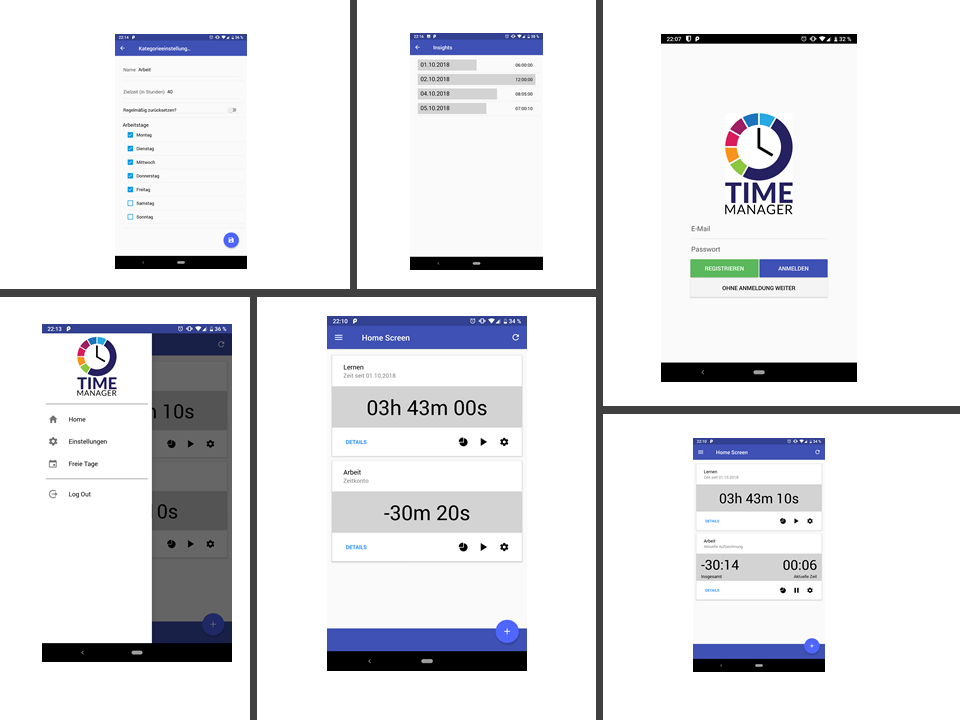
\includegraphics[width=\textwidth]{Final_App}
    \caption{Screenshots der Applikation}
    \label{fig:screenshots}
\end{figure}
\newpage
\section{Fazit}\label{sec:fazit}
Verbesserungen
\begin{itemize}
    \item Test
    \item Firestore Dokumente optimieren (Schreib-/Lesevorgänge)
     \item Löschen von Nutzer, Dokumenten, Kategorien
    \item Sortierung Kategorien-
\end{itemize}
\newpage

%\printacronyms{}
\printbibliography{}


\newpage
\appendix
\section{Datenbankstruktur}\label{app-datenbank}
    \begin{forest}
        pic dir tree,
        % where level=0{}{% folder icons by default; override using file for file icons
        %   directory,
        % },
        [/
            [users,directory
                [user1,file
                    [name]
                    [categories,directory
                        [categorie11,file
                            [name]
                            [total]
                            [target]
                            [...]
                            [times,directory
                                [2018-10-02T06:50:00.000Z,file
                                    [minutes]
                                    [started]
                                    [stopped]
                                ]
                                [...]
                            ]
                        ]
                        [...]
                    ]
                    [holidays,directory
                        [holiday1,file
                            [name]
                            [startDay]
                            [endDay]
                            [isFullDay]
                            [hours]
                        ]
                        [...]
                    ]
                ]
            ]
        ]
    \end{forest}

\section{LoginDeciderComponent}\label{app-LoginDecider}
\lstinputlisting[
    nolol,
    language=TypeScript
]{LoginDecider.tsx}

\section{Reflexion}\label{app-reflexion}
Ausgangssituation: Entwicklung mit JS (kein Typescript). Bezüglich React Native ausschließlich die Vorkenntnisse aus der Vorlesung.

Ziel der App: React(-native)
\end{document}
